\documentclass[11pt]{article}
\usepackage{array}
\usepackage{tabularx}
\usepackage{graphicx}
\usepackage{algorithm}
\usepackage{algorithmic}
\usepackage{pgfplotstable}
\usepackage{pgfplots}
\usepackage{filecontents}
\usepackage{amsmath}

\title{
	\textbf{IMS Final Project Report}
}

\author{Tobias Stahl \\ 10528199 \and Ioannis-Giounous Aivalis \\ 10524851 }

\begin{document}

\maketitle

\section{Introduction}
In this report we will present the process followed in order to create an end-to-end system for image classification. The product system will perform image classification on four classes of images (airplanes, motorbikes, faces and cars) using the bag-of-words approach.
%TODO - alternative to the next sentense ?
The report is layed out as follows, first we will explain the theoretical aspect of how our model works. Then we will get more into technical details about how our system can be divided into logical units.

\section{Bag-of-Words based Image Classification}
In this section we will shortly describe the method used in order to achieve the final system. For classification we used the Bag-of-words approach. The rest of this section is divided into logical parts explaining the pipeline of the system as it was implemented and the series of actions it takes to get from plain input images to calssified output images.

The Bag-of-words approach originates from the Natural Language Processing and Information Retrieval fields. According to this method the document is represented by a bag (multiset) of words consisting it. These bags are later used for training a classifier on those documents.

Similarly, in the image case, each image is represented as a bag of words, the words being-this time, the descriptors the image consists of. More specifically, each of the images descriptors is assigned a word from a predefined vocabulary. All of these terms will be explained in the remaining of this section. 

\subsection{Feature Extraction and Description}
\label{featureExtraction}
Each given image must undergo a preprocessing phase in order to be classified. In that directio, for each image that is processed by the system, a \emph{SiftImage} object is created. These objects now contain all the necessary information that might be required in future steps of the pipeline. More specifically, in the constructor of this class we extract various descriptors from which we will later have to decide which to use for training the classifier. These descriptors are obtained with:
\begin{itemize}
\item Dense SIFT: Extracted using the function \emph{vl\_dsift}\cite{vedaldi08vlfeat}. Note that due to the extensive size of the descriptors produced this way, we chose to select some of those at random (namely 300) to reduce the complexity of our system.
\item Key points SIFT: Extracted using the function \emph{vl\_sift}\cite{vedaldi08vlfeat}
\item RGB SIFT: For this SIFT we use the three different channels of the given image but we first eliminate the parts of the image with a low intensity, thus keeping only the interest points.
\item Normalized RGB SIFT: Similar to the previous sift but with normalized R,G and B values.
\item Opponent SIFT: Feature transformation on the opponent colors.
\end{itemize}

\subsection{Building Visual Vocabulary}
For this step we will process a subset of the training data in search of words to characterise the pictures. These words represent clusters of neighboring descriptors and are extracted using the k-means algorithm \cite{vedaldi08vlfeat} from the descriptors of the chosen subset.

This way, we can extract words that have the ability to characterise classes. It is these words that will later be used in order to characterise images by assigning one of those to each descriptor of a given image. In short these words determine the vocabulary.

\subsection{Quantize Features Using Visual Vocabulary}
Having obtained the visual vocabulary from the previous step we now proceed to characterizing each image as a bag-of-words. In order to do that we assign one word to each of the image's descriptors. This word is determined by finding the least "distance" from the words in the vocabulary.

\subsection{Classification}
In this section all the steps taken in the direction of training the classifier for the images will be analyzed. For the classifier we made use of the MATLAB Support Vector Machine interface implementation of \emph{libsvm}\cite{CC01a}

\subsubsection{Representing images by frequencies of visual words}
In order to train the classifier we need to provide it with representative data for each image. The convention taken here is that each image will be represented as a histogram of frequencies of the visual words it consists of. The histograms are first created and then normalized, to keep track of the possibly different number of features they consist of. An example histogram is shown in Figure \ref{wordhistogram}.

\begin{figure}[h!]
\centering
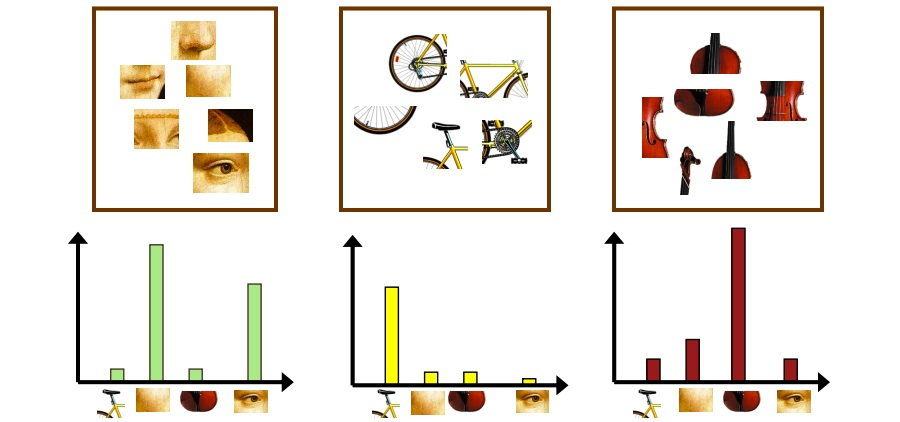
\includegraphics[scale=0.30]{wordhistogram.jpg}
\caption{Schematic representation of the bag-of-words system}
\label{wordhistogram}
\end{figure}

\subsubsection{Training the Classifier}
% vocImageRatio
For this task we need to provide the Support Vector Machine with training instances as well as with the label of those instances. To do that we simply go through the training folders in our data, sample some instances (the ammount of which will be thoroughly explained in the Evaluation section) and alongside those instances we create a class label vector which contains the corresponding class of the instance.

Now having the obtained the training instances we are ready to train a multi-class SVM for image classification.

\section{Experiments and Evaluation}
In this section we will show the experiments we conducted alongside the parameters we used per experiment as well as the results we obtained for each of the experiment setups. The experiment invariants are the following:
    \begin{itemize}
        \item Vocabulary image ratio := 20\% This means that the first 20\% of the images in the training folders are used in order to produce the vocabulary.
        \item Training image ratio := 80\% This ratio does not explicitly exist in our implementation, since we use the complement of the Vocabulary image ratio (above) to calculate it. We therefore choose to make use of all the training instances. Note here that the images used for the vocabulary are not used for training (the vocabulary and training instances do not overlap).
    \end{itemize}
The experiment variables are the following:
    \begin{itemize}
        \item SIFT type: As explained in Section \ref{featureExtraction} we provide five implementations of SIFT, each of which will yield different results.
        \item Vocabulary size: We have five given vocabulary sizes. Namely 400, 800, 1600, 2000, 4000 words. The size of the vocabulary determines the words that can be used to define a descriptor of an image.
    \end{itemize}

Table \ref{accuracies} provides a full overview of how the system performs in terms of accuracy under each different setting.

\begin{table}[h!]
    \centering
    \begin{tabular}{|c||ccccc|}
        \hline
             & Dense & KeyPoints & RGB  &   rgb    & Opponent \\
        \hline
        400  & 89.5  & 74.0      & 79.0 &   84.0   & 58.0 \\
        800  & 78.0  & 70.5      & 75.5 &   71.0   & 56.5 \\
        1600 & 72.5  & 65.5      & 57.5 &   64.5   & 48.0 \\
        2000 & 67.5  & 62.5      & 60.5 &   54.5   & 48.0 \\
        4000 & 56.5  & 54.0      & 49.0 &   53.0   & 46.0 \\
        \hline
    \end{tabular}
    \caption{Accuracy (\%) of the system subject to Vocabulary size and SIFT type}
\label{accuracies}
\end{table}

Further examination of the results Table reveals a trend as far as Vocabulary size is concerned, we can see that a bigger vocabulary results in worse performance. Size 400 seems to be the best candidate for this purpose. A bigger Vocabulary might produce coarse bags-of-words per image therefore encumbering the learning procedure.

As far as the SIFT types are concerned, we see a similar performance for (best performing) Dense and normalized rgb with the first achieving an accuracy close to 90\%. Keypoints seems to go head-to-head with RGB with RGB being superior for a smaller vocabulary whereas Keypoints seems to fluctuate less for vocabulary size 400 - 2000. Opponent seems to be the worst performing model with scores as low as 46\%, which is really bad for a 4-class only classification task.

A relativelly average performing model's performance is depicted in the confusion matrix \footnote{In a confusion matrix C; C(i,j) is defined as the count of observations known to be in group i but predicted to be in group j. This is a widely used visualization for classification issues and will be used in our report to depict model performances.} provided in Figure \ref{averageConf}. This is the performance for the system configuration: 800, Keypoints which achieved an overall accuracy score of 70.5\%.

% figure averageConf [h!] here
\begin{figure}[h!]
\centering
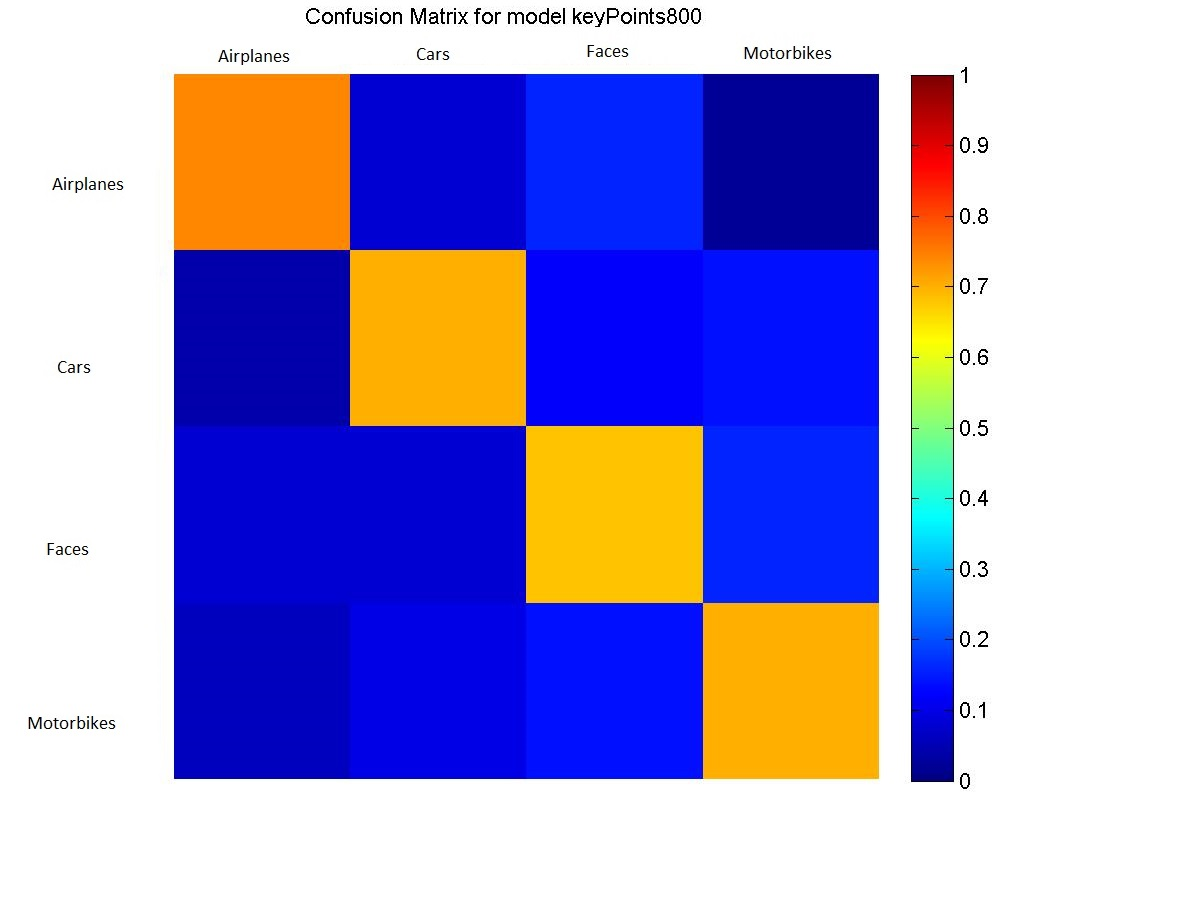
\includegraphics[scale=0.40]{averageConf.jpg}
\caption{Confusion Matrix of an average system configuration 800 Keypoints.}
\label{averageConf}
\end{figure}

% figure bestConf [h!] here
\begin{figure}[h!]
\centering
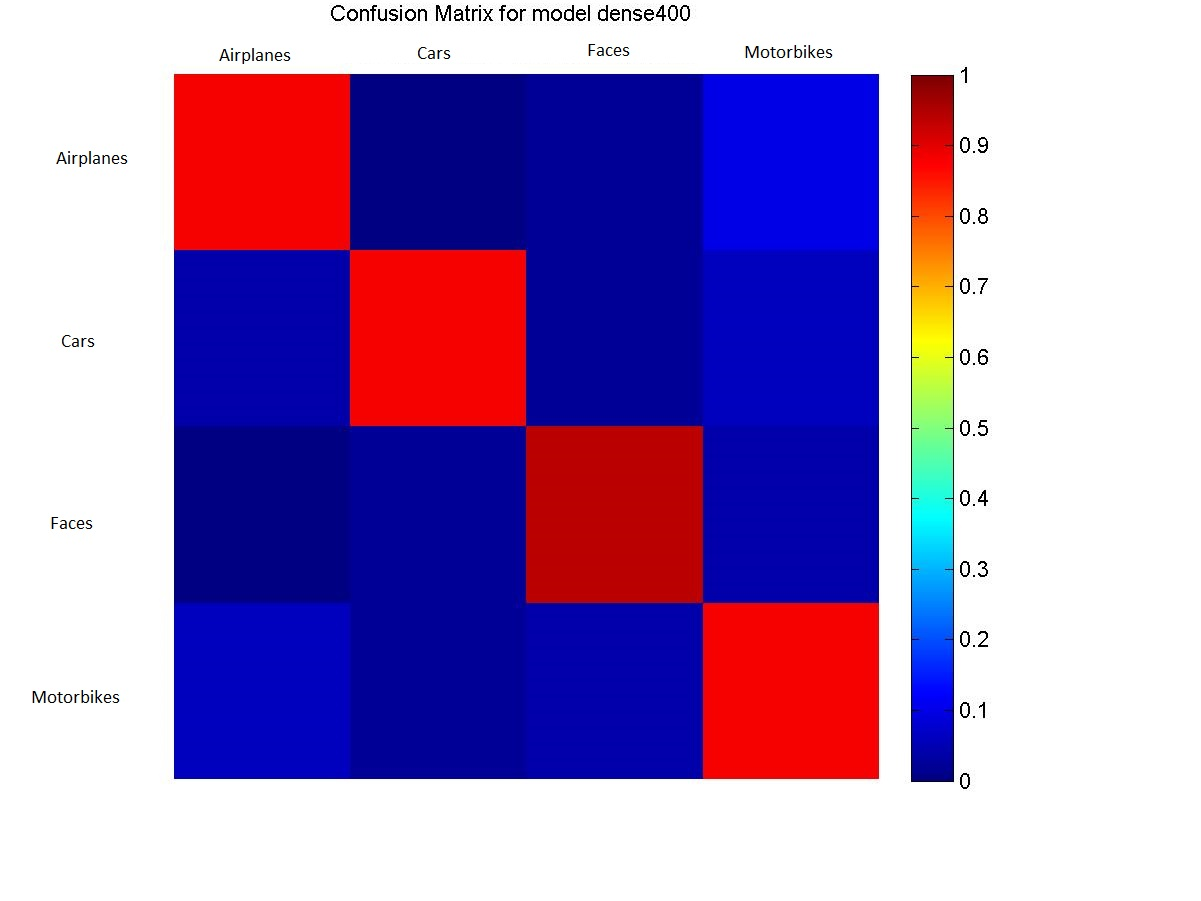
\includegraphics[scale=0.40]{bestConf.jpg}
\caption{Confusion Matrix of the best system configuration 400 Dense.}
\label{bestConf}
\end{figure}

We finally introduce the best performance for the system configuration 400, Dense (89.5\% accuracy). A more detailed version of this SVMs performance is introduced in the confusion matrix as shown in Figure \ref{bestConf}. Here we can see how well the system performs per class (true label versus predicted label). It is now visible that the labels \emph{Airplanes, Cars, Motorbikes} have the same accuracy (88.0 \%) whereas the classifier seems to perform best for the \emph{Faces} label (94.0\% accuracy).

\section{Conclusion}
Within this assignment we had the opportunity to implement a full end-to-end image classification system. We were introduced to the state-of-the-art techniques used for solving the problem at hand and used them in order to provide our solution to a four class image classifier. The solution we provided seems to achieve impressive results (even considering the small scale of our assignment) which is proof of the efficiency of the methods used.

\section{Future Work}
Due to the complexity of the system produced and the fact that our resources were limited we could not experiment with all the parameters of the experiment as much as we would have wanted. Interesting insights could be provided by tweaking the training sample count. Furthermore, experiments could be made to measure the performance of the multi-class SVM in comparisson to four 1-versus-all SVM classifiers. Lastly, the system built is robust to the input provided. In favor of that, experiments could be made with all kinds and sizes of inputs, so more classes could be utilized to see how it performs with different data. However this would require a significant ammount of time spent in preprocessing data which we did not have within the realms of this experiment.

\bibliography{biblio.bib}{}
\bibliographystyle{plain}
\end{document}